%-------------------------------------------------------------------------------
\section{Results}
\label{sec:results}
%-------------------------------------------------------------------------------

\begin{figure*}[t!]
    \centering
    \begin{subfigure}[b]{0.22\linewidth}
        \centering
        \includegraphics[width=\linewidth,trim={0 0 2cm 0.7cm},clip]
         {splitting-paper/figures/heatmaps/heatmap_tcp_cubic_10mbps.pdf}
        \captionsetup{skip=4pt}
        \caption{TCP CUBIC.}
        \label{fig:2d-heatmap:cubic-10}
    \end{subfigure}
    \begin{subfigure}[b]{0.22\linewidth}
        \centering
        \includegraphics[width=\linewidth,trim={0 0 2cm 0.7cm},clip]
         {splitting-paper/figures/heatmaps/heatmap_tcp_bbr1_10mbps.pdf}
        \captionsetup{skip=4pt}
        \caption{TCP BBRv1.}
        \label{fig:2d-heatmap:bbr1-10}
    \end{subfigure}
    \begin{subfigure}[b]{0.22\linewidth}
        \centering
        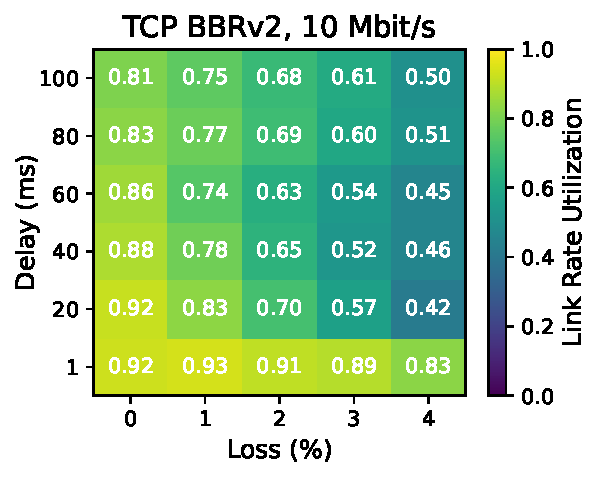
\includegraphics[width=\linewidth,trim={0 0 2cm 0.7cm},clip]
         {splitting-paper/figures/heatmaps/heatmap_tcp_bbr2_10mbps.pdf}
        \captionsetup{skip=4pt}
        \caption{TCP BBRv2.}
        \label{fig:2d-heatmap:bbr2-10}
    \end{subfigure}
    \begin{subfigure}[b]{0.22\linewidth}
        \centering
        \includegraphics[width=\linewidth,trim={0 0 2cm 0.7cm},clip]
         {splitting-paper/figures/heatmaps/heatmap_tcp_bbr3_10mbps.pdf}
        \captionsetup{skip=4pt}
        \caption{TCP BBRv3.}
        \label{fig:2d-heatmap:bbr3-10}
    \end{subfigure}
    \begin{subfigure}[b]{1cm}
        \includegraphics[width=1cm,trim={8cm 0 0 0},clip]
         {splitting-paper/figures/heatmaps/heatmap_tcp_bbr3_10mbps.pdf}
    \end{subfigure}
    \caption{The link rate utilization calculated as the ratio of achieved
     goodput to link rate for various TCP CCAs in an emulated network path, at
     various loss rates and one-way delays, at 10 Mbit/s. CUBIC is the
     most sensitive to loss and delay, while BBRv1 is the most aggressive and
     achieves the highest utilizations; BBRv2 and BBRv3 are more sensitive to
     loss than BBRv1 and utilization starts to suffer (left to right). CCAs
     tend to achieve lower utilizations, though higher absolute goodputs, as
     the link rate increases (\Cref{sec:appendix}). Median of $n=20$ trials.}
    \label{fig:2d-heatmap}
\end{figure*}


In our emulation measurement study, we aim to answer three questions to gain a
more comprehensive understanding of the relevance of connection-splitting with
modern networks:

\begin{enumerate}[noitemsep]
    \item Has the model-based BBR algorithm made the throughput enhancements of
     connection-splitting obsolete?
    \item Are there classes of network settings where BBR benefits significantly
     from splitting but CUBIC does not?
    % \thea{I am still not totally convinced by this claim as a "headline" and
    %  think the network path "classes" are more interesting.}
    \item How does CCA implementation impact end-to-end behavior, and therefore split
     behavior?
\end{enumerate}

\noindent To recap our measurement methodology, we have a method for
 measuring the throughput of TCP connections in emulation both with and without a
 transparent PEP. We also have the ability to estimate throughput both with and
 without a generic connection splitter, for both TCP and QUIC, based on
 knowledge of the network model of each path segment, and the measured end-to-end
 throughput on each segment.

For our analysis, we cache measurements for the end-to-end network parameters
in \Cref{tab:parameters} and the congestion control schemes in \Cref
{tab:cca-implementations}. We also run experiments in the two-segment network topology
to validate some of these predictions. Raw data for the end-to-end
behavior of each CCA implementation are available in \Cref{sec:appendix}.
Our emulation benchmarks are also publicly available on GitHub: \url{https://github.com/StanfordSNR/connection-splitting}.

\subsection{Finding: Splitting has become significantly more beneficial to TCP
 BBR since it was initially released in 2016.}

Has the model-based BBR algorithm made the throughput enhancements of
connection-splitting obsolete? We find this line of thought has some truth
with the initial release of TCP BBRv1 in 2016. But as the BBR algorithm has
evolved into BBRv2 in 2019 and now BBRv3 in 2023, it has also evolved to behave
more conventionally in the sense that it benefits from being split---just like
more traditional, loss-based congestion control schemes such as CUBIC.

% \begin{table}[t!]
  \centering
\begin{tabular}{ r l l }
  \toprule
    \textbf{Fig.} & \textbf{Segment 1} & \textbf{Segment 2} \\
    \midrule
    \ref{fig:bbr-over-time:class1} & 1ms, 20 Mbit/s, 4\% & 100ms, 20 Mbit/s, 0\% \\
    \ref{fig:bbr-over-time:class2} & 100ms, 20 Mbit/s, 2\% & 1ms, 20 Mbit/s, 2\%\\
    \ref{fig:bbr-over-time:class3} & 40ms, 40 Mbit/s, 2\% & 40ms, 40 Mbit/s, 2\%\\
\bottomrule
\end{tabular}
  \caption{\label{tab:network-setting-params} The propagation delay, link rate,
   and random loss for each path segment of the three scenarios in \Cref
   {fig:bbr-over-time}. \gina{Need to make consistent the use of link rate vs.
   bandwidth etc.}}
\end{table}


\Cref{fig:bbr-over-time} shows three different network settings in which BBRv2
and BBRv3 show significant throughput gains from connection-splitting.
 When BBRv1 was released, its throughput both with and
 without the connection-splitter were roughly the same, and nearly achieved the
 bottleneck link rate. With BBRv2 and BBRv3, the end-to-end throughput
 drastically deteriorated, behaving more like CUBIC than BBRv1. However, the
 split throughput remained relatively high, suggesting that BBRv3 today would
 still benefit from connection-splitting.

\paragraph{Analysis.}
To explore why CUBIC and BBRv3 benefit from splitting but BBRv1 does not, we
analyze end-to-end throughputs of each CCA and apply the split throughput
heuristic (\Cref{fig:heuristic}). As described in \Cref{sec:heuristic}, this
methodology allows us to study split settings by measuring the much smaller
parameter space of end-to-end connections.
We find that connection-splitting is likely to improve throughput on lossy
paths for CUBIC, BBRv2, and BBRv3 connections, but not for BBRv1.

\Cref{fig:2d-heatmap} visualizes our cached end-to-end measurements as link rate
 utilization heatmaps of loss vs. delay.
 Here is an example for how to interpret these graphs using \Cref
 {fig:2d-heatmap:bbr3-10}. The top-left cell represents a 100 ms 0\% segment
 with 0.82 utilization of the 10 Mbit/s link rate, and the bottom-right cell
 represents a 1 ms 4\% segment with 0.85 utilization of the 10 Mbit/s link
 rate. The predicted split utilization of a network path composed of these two
 segments is just 0.82, the minimum. The two cells compose to the top-right
 cell, which represents a 100 ms 4\% 10 Mbit/s segment with an end-to-end
 utilization of 0.49. Since $0.82>0.49$, we say that splitting has improved the
 throughput of this network path.

BBRv1 achieves high link rate utilization in all settings (\Cref
{fig:2d-heatmap:bbr1-10}), showing it has little to gain from splitting.
In fact, previous studies have shown that BBRv1 achieves $\approx\!85\%$
link utilization regardless of loss (same as our findings) before it reaches
a cliff point at around 20\% loss~\cite{cao2019use,cardwell2017bbr}.
This may be why it appears that splitting in lossy settings is now obsolete with BBR.
However, one should note that BBRv1's high throughput has long been attributed
to its aggressiveness and unfairness to legacy algorithms~\cite
{ware2019modeling,cao2019use}, which is what led to the changes in BBRv2 and
BBRv3.

While BBRv2 is a large departure from BBRv1, BBRv3 has been described as BBRv2
with bugfixes and performance tuning~\cite{cardwell2024bbrv3-ietf119}, which
supports why the two are so similar. We focus on BBRv3 since Google hopes to
now deprecate BBRv2~\cite{cardwell2024bbrv3-ietf119}.

% Unlike BBRv1, BBRv3 uses loss as a congestion signal. Indeed, BBRv3's end-to-end
% throughput suffers under high loss (\Cref{fig:2d-heatmap:bbr3-10}), though to a
% lesser extent than CUBIC (\Cref{fig:2d-heatmap:cubic-10}). Our results reflect
% existing findings of lower utilization in BBRv2 and BBRv3~\cite
% {datta2023replication,song2021understanding,zeynali2024promises}.
BBRv3 is more sensitive to loss than its previous versions (\Cref
{fig:2d-heatmap:bbr3-10}), and more similar to CUBIC (\Cref
{fig:2d-heatmap:cubic-10}) in that there exist scenarios where end-to-end
throughput suffers.
These reflect existing findings of lower utilization in BBRv2 and BBRv3~\cite
{datta2023replication,song2021understanding,zeynali2024promises}.
Based on the heuristic, it is clear that in some lossy networks
such as the ones empirically evaluated in \Cref{fig:bbr-over-time},
connection-splitting
can significantly increase the throughput of BBRv3 connections.
It is possible that the BBR algorithm continues to evolve in this direction
given that BBR's unfairness remains contentious today~\cite
{datta2023replication,zeynali2024promises}.

\paragraph{Summary.}

While BBR may not have benefited from splitting with the release of ``v1'' in 2016, BBRv2 and
now BBRv3 have evolved to behave more conventionally---similar to traditional,
loss-based CCAs such as CUBIC---in the sense that they \textit{do}. Even
so-called ``model-based'' congestion control algorithms seem to now react to
loss as a congestion signal, as the BBR algorithm continues to evolve.

\subsection{Finding: There exist classes of network paths where TCP BBRv3 would
 significantly benefit from splitting but TCP CUBIC would not.}

Are there new classes of network settings where BBR benefits significantly from
splitting but CUBIC does not? We want to understand the network settings in
which a congestion control scheme is not able to achieve practical bottleneck
link rate utilizations end-to-end, but is with a connection-splitter.

We find that while splitting benefits BBRv3 in all the same scenarios as CUBIC,
it also has the potential to benefit BBRv3 in many \textit{new} scenarios.
In addition to edge deployments with a lossy last-mile, BBRv3
also benefits from splitting in scenarios where there is loss on both path
segments, and when the connection-splitter is located farther from the edge.
We partition these scenarios into three classes of network settings:

\begin{enumerate}[label=\Roman*.,noitemsep]
\item Paths with asymmetric delay and a lossy last-mile,
\item Lossy paths with asymmetric delay,
\item Lossy paths with more symmetric delay.
\end{enumerate}

\noindent \Cref
 {fig:bbr-over-time:class1,fig:bbr-over-time:class2,fig:bbr-over-time:class3}
represent network settings in each class, respectively.
``Asymmetric'' refers to the delays on the two path segments.
These emulations empirically demonstrate that CUBIC only benefits in the first
class, while BBRv3 benefits in all three.
BBRv1 does not need splitting in any context.

\paragraph{Analysis.}
To identify which network paths benefit from connection-splitting and where
along the paths PEPs should be deployed, we apply the
heuristic (\Cref{fig:heuristic}).
For each CCA, we conduct an exhaustive search of the $15 \cdot 21 \cdot 25 =
7875$ combinations of settings within our parameter space (\Cref
{tab:parameters}), and efficiently predict the split and end-to-end throughputs.

We filter on the predicted throughputs for network settings where splitting improves end-to-end throughput by
at least $3\times$, and where the split connection utilizes at least half the
bottleneck link rate (\Cref{tab:network-path-analysis}). BBRv1 does not meet
these criteria is any scenarios, and the theoretical connection-splitter is
unable to improve the throughput of BBRv1 by even $50\%$. CUBIC and BBRv3 meet
these criteria in 942 and 188 scenarios, respectively. CUBIC benefits from
splitting in more scenarios because its end-to-end utilization is more
frequently low, so it more frequently has a large split improvement.

\begin{table}[t!]
  \centering
\begin{tabular}{ r l l l }
  \toprule
    \textbf{Filter} & \textbf{BBRv1} & \textbf{CUBIC} & \textbf{BBRv3} \\
    \midrule
    Initial & 7875 & 7875 & 7875 \\
    Split imprvmnt. $>3\times$ & 0 & 2231 & 234 \\
    Split utilization $>0.5$ & 0 & 942 & 188 \\
    \midrule
    Asymmetric, last-mile & 0 & 942 & 38 \\
    Asymmetric, lossy & 0 & 0 & 72 \\
    Symmetric, lossy & 0 & 0 & 78 \\
    \bottomrule
\end{tabular}
  \caption{\label{tab:network-path-analysis} An exhaustive search of network
   paths and their PEP locations that benefit from splitting for each CCA, and
   the number of filtered settings that belong to each class.}
  \vspace{-0.4cm}
\end{table}


Since the distribution of network paths in our parameter space does not reflect
any meaningful real world distribution, we are more interested in the \textit
{classes} of network settings that benefit from splitting. We realized
that \textit{all} of the relevant network settings for CUBIC can be clustered
into Class I, as network paths where one path segment has $1$ ms delay and
non-zero loss, and the other has $>1$ ms delay and $0\%$ loss. However, Class
I only accounts for $21\%$ of the relevant network settings for BBRv3. We
identify Class II, which is the same as I, except both path segments have
non-zero loss. Class III is the same as II, except both path segments have
$>1$ ms delay. We used the results to select three representative network
settings to empirically evaluate in \Cref{fig:bbr-over-time}.

Intuitively, we can understand why BBRv3 benefits more from splitting in lossy
scenarios than CUBIC based on how it reacts to loss and delay (\Cref
{fig:2d-heatmap:bbr3-10}). BBRv3's sensitivity to loss
and delay is more gradual than abrupt, so it is more likely to benefit when
splitting a lossy, high-delay network path in any way. In comparison, CUBIC's
throughput falls off a cliff for many of these segmentations.

\paragraph{Discussion.}
Do these results reflect where PEP deployments have been useful in the real
world? Connection-splitters have traditionally been found in satellite,
cellular, and Wi-Fi networks with a wireless link or rate policer~\cite
{edeline2019bottomup,honda2011still}. This resembles Class I, where the
network path consists of a lossy last-mile, and a reliable Internet path
segment. It makes sense then for PEPs to be traditionally located at the edge
to address the issues of loss-based schemes~\cite
{cloudsplitting2010,rfc3135,farkas2012splittcp}. We expect these PEPs to
similarly benefit BBRv3 in the same locations.

In Classes I and II, asymmetric delay can be severe in low-resource networks
in addition to wireless last-mile links;
Consider, for example, regions with no IXPs in which a significant proportion
of Internet traffic travels internationally.

For Classes II and III, satellite (and also wireless ad-hoc)
networks are known for
having lossy ``middle-miles''~\cite{kuhn2021quic-over-sat,border2022evaluating,pirovano2013new,cloudsplitting2010}.
This can be due to bad weather, fast-moving satellites, and
long-distance radio waves, etc.
Since CUBIC does not trivially benefit from splitting in these scenarios, the
traditional solution has been to split the connection at multiple points and to
use an FEC-based or other proprietary protocol in the satellite backhaul~\cite
{cloudsplitting2010,border2022evaluating,rfc3135}.
Our results suggest such an invasive solution may not be necessary for BBRv3.

How could this inform the deployment of connection-splitting PEPs?
With the caveat that futher exploration is required to understand how the
heuristic extrapolates to the real world, one idea is to
determine where to deploy PEPs along an existing network path for maximum
benefit especially as congestion-control schemes evolve.
Another idea is given the location of a PEP, determine which connections going
through the PEP would most benefit based on knowledge of each connection's
network path.
We leave network operators to decide how best to model their networks and apply
the heuristic to evaluate potential PEP deployments.

% \gina{Expand on the impact of these findings especially for new types of GEO and
%  LEO satellite networks. I think cellular network operators will be skeptical of the
%  relevance of these findings (they don't really believe in loss), but satellite
%  network operators may be more sympathetic.}

\paragraph{Summary.}
While TCP CUBIC only benefits from connection-splitting when the PEP is located
at the lossy last-mile, TCP BBRv3 can also benefit when there is loss on both
sides of the PEP and when there are longer propagation delays. This suggests
that TCP connections using BBRv3 should benefit from splitters at the same
locations as for CUBIC, and also that traditional methods used to
address loss in the middle-mile could use simple connection-splitting instead.
We believe this method of analyzing useful network paths and PEP placements for
connection-splitting can be extended to model new types of networks, especially
in space.

% \subsection{Finding: BBR's end-to-end behavior depends on implementation, and
%  evaluations of connection splitting should likewise take implementation into
%  account.}
\subsection{Finding: QUIC implementations of the same congestion control schemes
 vary significantly, and further differ from Linux's TCP implementations.}

\begin{figure*}[t!]
    \centering
    \begin{subfigure}[b]{0.22\linewidth}
        \centering
        \includegraphics[width=\linewidth,trim={0 0 2cm 0.7cm},clip]
        {splitting/figures/heatmaps/heatmap_tcp_bbr3_10mbps.pdf}
        \captionsetup{skip=4pt}
        \caption{TCP, BBRv3}
        \label{fig:splitting:quic:tcp-bbr3}
    \end{subfigure}
    \begin{subfigure}[b]{0.22\linewidth}
        \centering
        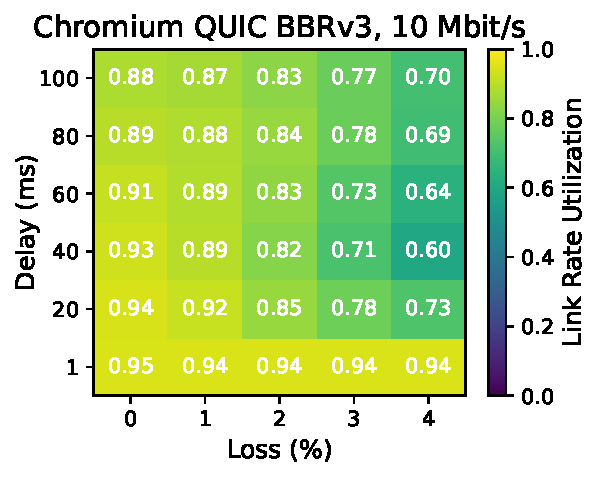
\includegraphics[width=\linewidth,trim={0 0 2cm 0.7cm},clip]
        {splitting/figures/heatmaps/heatmap_quic_bbr3_10mbps.pdf}
        \captionsetup{skip=4pt}
        \caption{Google, BBRv3}
        \label{fig:splitting:quic:google-bbr3}
    \end{subfigure}
    \begin{subfigure}[b]{0.22\linewidth}
        \centering
        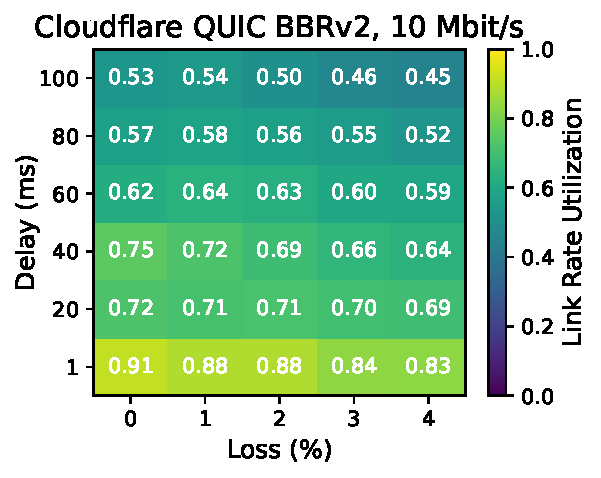
\includegraphics[width=\linewidth,trim={0 0 2cm 0.7cm},clip]
        {splitting/figures/heatmaps/heatmap_quiche_bbr2_10mbps.pdf}
        \captionsetup{skip=4pt}
        \caption{Cloudflare, BBRv2}
        \label{fig:splitting:quic:cloudflare-bbr2}
    \end{subfigure}
    \begin{subfigure}[b]{0.22\linewidth}
        \centering
        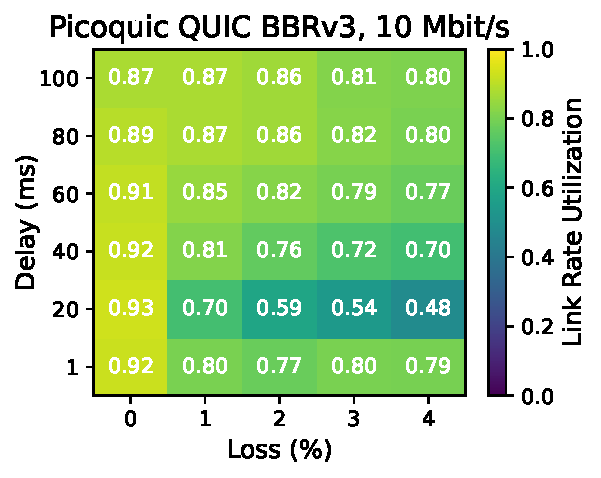
\includegraphics[width=\linewidth,trim={0 0 2cm 0.7cm},clip]
        {splitting/figures/heatmaps/heatmap_picoquic_bbr3_10mbps.pdf}
        \captionsetup{skip=4pt}
        \caption{\texttt{picoquic}, BBRv3}
        \label{fig:splitting:quic:picoquic-bbr3}
    \end{subfigure}
    \begin{subfigure}[b]{0.9cm}
        \includegraphics[width=0.9cm,trim={8cm 0 0 0},clip]
        {splitting/figures/heatmaps/heatmap_tcp_bbr3_10mbps.pdf}
        \vspace{0.08cm}
    \end{subfigure}
    
    \begin{subfigure}[b]{0.22\linewidth}
        \centering
        \includegraphics[width=\linewidth,trim={0 0 2cm 0.7cm},clip]
        {splitting/figures/heatmaps/heatmap_tcp_bbr1_10mbps.pdf}
        \captionsetup{skip=4pt}
        \caption{TCP, BBRv1}
        \label{fig:splitting:quic:tcp-bbr1}
    \end{subfigure}
    \begin{subfigure}[b]{0.22\linewidth}
        \centering
        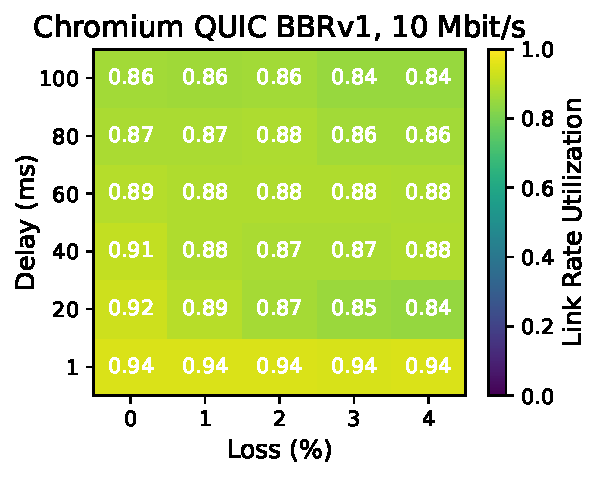
\includegraphics[width=\linewidth,trim={0 0 2cm 0.7cm},clip]
        {splitting/figures/heatmaps/heatmap_quic_bbr1_10mbps.pdf}
        \captionsetup{skip=4pt}
        \caption{Google, BBRv1}
        \label{fig:splitting:quic:google-bbr1}
    \end{subfigure}
    \begin{subfigure}[b]{0.22\linewidth}
        \centering
        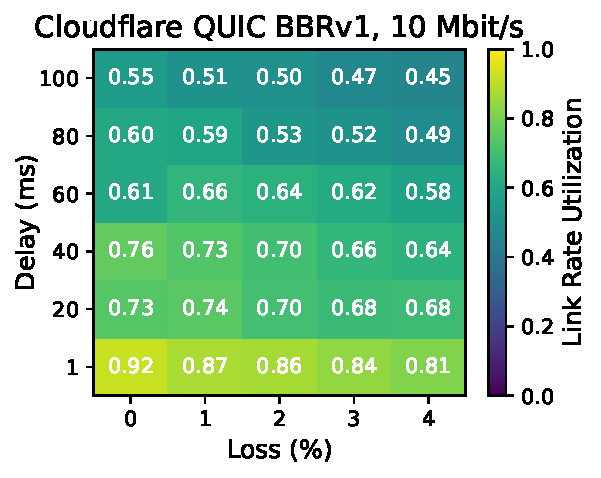
\includegraphics[width=\linewidth,trim={0 0 2cm 0.7cm},clip]
        {splitting/figures/heatmaps/heatmap_quiche_bbr1_10mbps.pdf}
        \captionsetup{skip=4pt}
        \caption{Cloudflare, BBRv1}
        \label{fig:splitting:quic:cloudflare-bbr1}
    \end{subfigure}
    \begin{subfigure}[b]{0.22\linewidth}
        \centering
        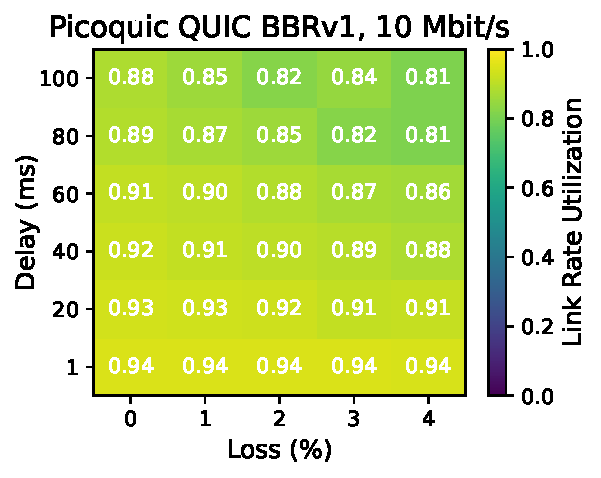
\includegraphics[width=\linewidth,trim={0 0 2cm 0.7cm},clip]
        {splitting/figures/heatmaps/heatmap_picoquic_bbr1_10mbps.pdf}
        \captionsetup{skip=4pt}
        \caption{\texttt{picoquic}, BBRv1}
        \label{fig:splitting:quic:picoquic-bbr1}
    \end{subfigure}
    \begin{subfigure}[b]{0.9cm}
        \includegraphics[width=0.9cm,trim={8cm 0 0 0},clip]
        {splitting/figures/heatmaps/heatmap_tcp_bbr1_10mbps.pdf}
        \vspace{0.08cm}
    \end{subfigure}

    \begin{subfigure}[b]{0.22\linewidth}
        \centering
        \includegraphics[width=\linewidth,trim={0 0 2cm 0.7cm},clip]
        {splitting/figures/heatmaps/heatmap_tcp_cubic_10mbps.pdf}
        \captionsetup{skip=4pt}
        \caption{TCP, CUBIC}
        \label{fig:splitting:quic:tcp-cubic}
    \end{subfigure}
    \begin{subfigure}[b]{0.22\linewidth}
        \centering
        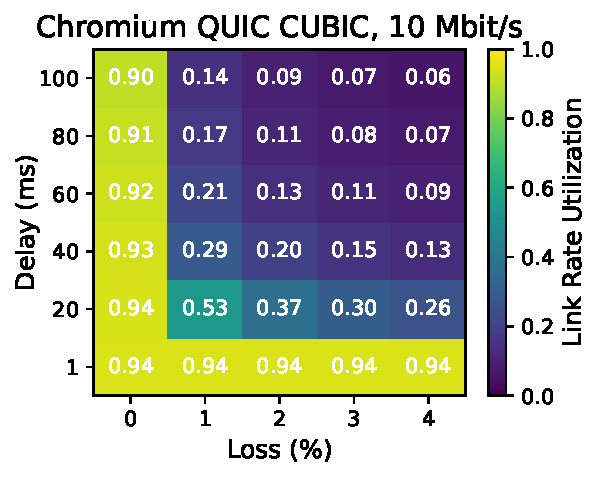
\includegraphics[width=\linewidth,trim={0 0 2cm 0.7cm},clip]
        {splitting/figures/heatmaps/heatmap_quic_cubic_10mbps.pdf}
        \captionsetup{skip=4pt}
        \caption{Google, CUBIC}
        \label{fig:splitting:quic:google-cubic}
    \end{subfigure}
    \begin{subfigure}[b]{0.22\linewidth}
        \centering
        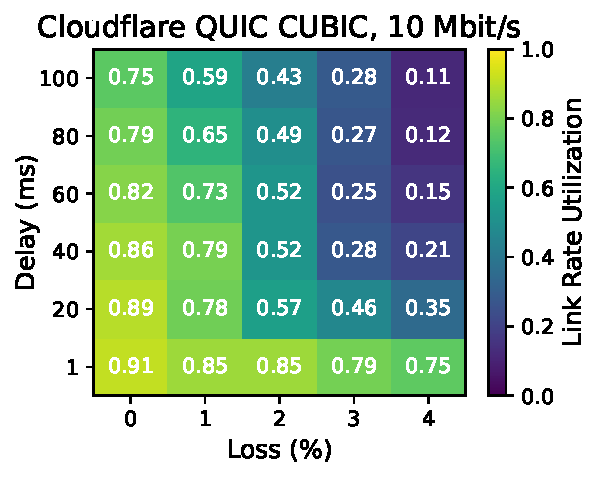
\includegraphics[width=\linewidth,trim={0 0 2cm 0.7cm},clip]
        {splitting/figures/heatmaps/heatmap_quiche_cubic_10mbps.pdf}
        \captionsetup{skip=4pt}
        \caption{Cloudflare, CUBIC}
        \label{fig:splitting:quic:cloudflare-cubic}
    \end{subfigure}
    \begin{subfigure}[b]{0.22\linewidth}
        \centering
        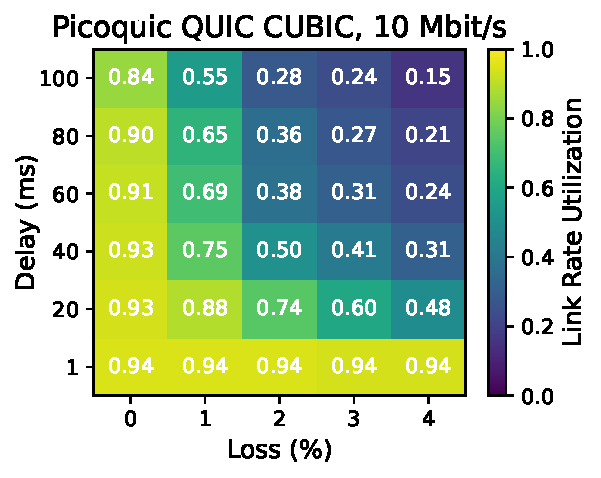
\includegraphics[width=\linewidth,trim={0 0 2cm 0.7cm},clip]
        {splitting/figures/heatmaps/heatmap_picoquic_cubic_10mbps.pdf}
        \captionsetup{skip=4pt}
        \caption{\texttt{picoquic}, CUBIC}
        \label{fig:splitting:quic:picoquic-cubic}
    \end{subfigure}
    \begin{subfigure}[b]{0.9cm}
        \includegraphics[width=0.9cm,trim={8cm 0 0 0},clip]
        {splitting/figures/heatmaps/heatmap_tcp_cubic_10mbps.pdf}
        \vspace{0.08cm}
    \end{subfigure}

    \caption{Heatmaps for three QUIC implementations of BBRv3 (or BBRv2), BBRv1,
     and CUBIC showing link rate utilization calculated as the ratio of
     achieved goodput to link rate, compared to Linux TCP. The heatmaps are
     shown at various loss rates and one-way delays with a fixed link rate of
     10 Mbit/s. User-space QUIC is not CPU-limited, achieving high utilizations
     at 1 ms delay and 0\% loss. The QUIC implementations are Google \texttt
     {quiche}, Cloudflare, and a minimalist implementation
     based on the IETF spec called \texttt{picoquic}. Median of $n=20$
     trials.}
    \label{fig:splitting:quic}
\end{figure*}


How does CCA implementation impact end-to-end behavior, and therefore split
behavior? Might claims about ``split throughput'' depend not just on the CCA,
but also the \textit{implementation} and/or the transport protocol
on top of it?

For our initial study, we compared end-to-end throughput for four open-source
implementations each of CUBIC, BBRv1, and BBRv2/3; one using TCP and three
using QUIC. We find that the end-to-end behavior of each CCA varies by
implementation in both baseline throughput and sensitivity to loss and delay.
To evaluate the split behavior of QUIC, instead of creating a custom and
explicit connection-splitting PEP for each QUIC implementation, we apply the
split throughput heuristic and argue that these implementations
will likewise respond differently to connection-splitting PEPs.

% We think this is important to answer with the rise of different QUIC
% implementations~\cite{marx2020same}, as it remains contentious whether
% encrypted protocols should receive in-network assistance~\cite
% {yuan2024sidekick}.
% This makes it frustrating to directly compare QUIC and TCP.

\Cref{fig:quic} visualizes the end-to-end behavior of these schemes.
We highlight that the Cloudflare and \texttt
 {picoquic} CUBIC implementations are less sensitive to loss than Google or
 TCP; the former may benefit from splitting in more classes of network settings
 than the latter. Additionally, their BBR implementations exhibit non-uniform
 behavior, suggesting a non-uniform response to
 connection-splitting. These variations indicate that the benefits of
 in-network assistance should be considered along with not just the CCA but its
 specific implementations.

% We believe it is important to consider CCA \textit{implementation}, along with
% CCA choice, application-level behavior~\cite{philip2024prudentia}, transport
% protocol mechanisms~\cite{marx2020same}.

\paragraph{Analysis.}

The Google QUIC (\Cref{fig:quic:google-bbr1,fig:quic:google-bbr3,fig:quic:google-cubic})
and TCP (\Cref{fig:quic:tcp-bbr1,fig:quic:tcp-bbr3,fig:quic:tcp-cubic})
implementations are most similar to each other for each CCA.
This is reasonable if we take the community-based CUBIC implementation in
Linux to be the standard, and considering that Google contributed to the Linux
BBR implementations. In general, Google QUIC achieves slightly higher
utilization than Linux TCP.

The Cloudflare QUIC BBR implementations (\Cref{fig:quic:cloudflare-bbr1,fig:quic:cloudflare-bbr2})
exhibit profoundly different behavior from Linux TCP in baseline performance.
Note that Cloudflare uses BBRv1 for TCP but their use of BBR in QUIC
is experimental. Anecdotally, a
Cloudflare employee has expressed difficulty making
their BBR implementation performant, having to reverse engineer
the Linux kernel~\cite{cardwell2024bbrv3-ietf119-qna}. Given the wide adoption
of BBRv1 for TCP at many CDNs~\cite{ware2024ccanalyzer}, we expect it to
be desirable yet challenging for these same companies to correctly incorporate
BBRv3 into their QUIC stacks in the coming years.
% Maybe cite narayan2018restructuring

The \texttt{picoquic} BBR implementations (\Cref{fig:quic:picoquic-bbr1,fig:quic:picoquic-bbr3})
are more similar to Linux TCP, although its BBRv3 implementation seems to have
a contradicting reaction to delay.
We note that \texttt{picoquic} is intended for experimental use in the
IETF~\cite{picoquic}. It is important then to understand its congestion control
behavior if it is to be used to evaluate
IETF proposals. We believe its differences from Linux TCP warrant further
exploration, but perhaps also that the ongoing standardization efforts of BBR
in the IETF~\cite{cardwell2024bbr-ietf-draft} indicate
that there is no monolith yet of ``the BBR algorithm.''

The Cloudflare QUIC and \texttt{picoquic} implementations of CUBIC
(\Cref{fig:quic:cloudflare-cubic,fig:quic:picoquic-cubic}) interestingly
both exhibit a more gradual degradation in response to loss and delay than Linux TCP
(\Cref{fig:quic:tcp-cubic}). We
find this harder to explain, given that TCP CUBIC has been around since 2006,
and perhaps can be attributed to transport protocol mechanisms in QUIC.
Nevertheless, this indicates that it is important to understand the
behavior of a CCA in the context of its entire
implementation.

\begin{figure}[t!]
    \centering
    \begin{subfigure}[b]{\linewidth}
        \centering
        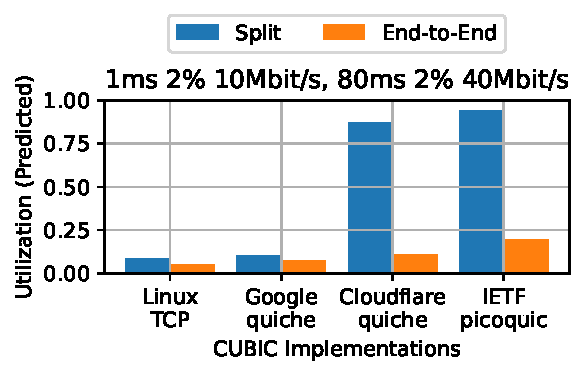
\includegraphics[width=0.8\linewidth]
         {splitting-paper/figures/network_path_analysis/network_path_analysis_10_40_1_80_2_2.pdf}
        \captionsetup{skip=0pt}
        \caption{Some QUIC CUBIC implementations can benefit in new network
         classes where TCP CUBIC could not.}
        \label{fig:quic-predictions:cubic}
    \end{subfigure}
    \begin{subfigure}[b]{\linewidth}
        \centering
        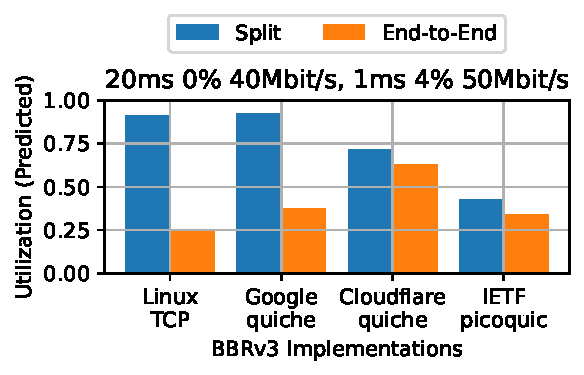
\includegraphics[width=0.8\linewidth]
         {splitting-paper/figures/network_path_analysis/network_path_analysis_40_50_20_1_0_4.pdf}
        \captionsetup{skip=0pt}
        \caption{The various BBRv3 implementations have non-uniform end-to-end
         behavior and no clear resulting split behavior.}
        \label{fig:quic-predictions:bbr3}
    \end{subfigure}
    \caption{Predicted bottleneck link rate utilizations calculated from the
     predicted end-to-end and split throughputs of the TCP and QUIC
     implementations, on two different network path segments. End-to-end
     behavior of each CCA varies significantly by implementation.}
    \label{fig:quic-predictions}
\end{figure}


\Cref{fig:quic-predictions} applies the heuristic to show how split behavior
can vary for CCA implementations with different end-to-end behaviors.
Some QUIC CUBIC implementations
benefit in new network settings where TCP CUBIC does not, while the various
QUIC BBRv3 implementations exhibit non-uniform end-to-end behavior and thus no
clear trend in split behavior.

% On the other hand, Cloudflare's implementations exhibit profoundly different
% behavior. Cloudflare's quic-CUBIC implementation appears more aggressive than
% those in Linux or Chromium. As expected, quic-BBRv1 and v2 are less responsive
% to loss than CUBIC, but goodputs trend \textit{lower} than in quic-CUBIC. This
% may reflect that Cloudflare's quic-BBR implementations are relatively new \cite
% {} and, as far as we are aware, not yet deployed in production \cite{}. \thea
% {Could add observation of the BBR code possibly introducing some additional
% loss, but we confirmed no full send buffers or loss on interfaces.}

\paragraph{Discussion.}

Why do we believe we can extrapolate split behavior from the end-to-end behavior
of QUIC? Previous studies explore the effects of QUIC's transport protocol
mechanisms in such a case~\cite{kosek2022quicpep,thomas2019google}. They find
that the effects of zero-RTT connection establishment with regards to
long-lived throughput to be minimal, and stream multiplexing to be mutually
beneficial in both scenarios. Further studies can clarify the interactions
between CCAs and transport mechanisms.

How do we know that the difference in behavior is due to the congestion control
implementation and not other transport protocol mechanisms? Well, we
don't, and there is known to be significant variance in the features supported
by different QUIC implementations~\cite{marx2020same}.
However, we find it intuitive that congestion control would be a major factor in
the measured sustained goodput of a bulk file transfer.

The divergence in QUIC implementations is not so dissimilar from that of TCP at
a similar state of evolution~\cite{allman1999effective}, but there are still
some fundamental differences. With QUIC implementations in userspace, there is
a larger diversity of implementations that are easier to tune for a specific
application metric, as opposed to correctness or fairness from a
congestion-control point of view. These algorithms are also highly
parameterized, with no standard nor test suite, so it's not surprising that the
implementations differ.

If there is reason to believe
that QUIC is losing out on throughput by not connection-splitting, then there
will continue to be research on how to achieve the same benefits without
ossification~\cite{kosek2023secure,yuan2024sidekick,kramer2021masquepep,yuan2022sidecar}.
The heuristic helps us understand the theoretical achievable
throughput with a simple connection-splitter, or even by combining multiple
end-to-end congestion control schemes.
In addition to research, this could motivate privacy-minded proposals in the Internet
standards community to also view themselves as potential deployment opportunities
for private PEPs~\cite{kosek2021masque,sattler2022towards,rfc9297,rfc9298}.
% For example, MASQUE is an explicit
% connection-splitter~\cite{kosek2021masque}, and PACUBIC is a path-aware
% congestion control algorithm that uses signals provided by network
% intermediaries in the Sidekick protocol~\cite{yuan2024sidekick}.
% While we do not think QUIC will ever have transparent connection-splitting
% proxies due to ossification, these proposals demonstrate that other methods of
% in-network assistance are possible.

% The analysis makes two assumptions: that congestion control is the major factor
% in explaining differences in end-to-end behavior, and that the congestion
% control and not other transport protocol mechanisms are the most important
% factors in extrapolating split performance.

% \begin{figure}[t!]
    \centering
    \includegraphics[width=\linewidth,height=100pt]{example-image-a}
    \caption{BBRv1 performance on 13 Linux kernels between 2016 and 2024.}
    \label{fig:bbr1-over-time}
\end{figure}


Another application of analyzing CCA implementations is to analyze the Linux TCP
implementations of BBR \textit{within} a major version over time. We did
this analysis with BBRv1 on 13 Linux kernels between 2016 and 2024, but found
no significant variance. However, given the dynamic nature of BBR and the
Linux networking stack, it
is possible there will still be changes to the split behavior of TCP in the future.

% \thea{Not sure where this belongs?} Recognizing that there have been changes to
%  both BBRv1 and the Linux networking stack \cite{} since 2016, we repeated
%  BBRv1 experiments in 13 Linux kernels between 2016 and 2024. We confirm that
%  BBRv1 does not meaningfully benefit from connection-splitting in any release
%  or network emulation. There are subtle differences in earlier versions
%  (e.g., higher standard deviation across multiple trials), but the irrelevance
%  of connection splitting is the same. can be used to evaluate the cca in the
%  past (and in the future). Plot the splittability of the congestion control
%  algorithms over time and how different iterations of it look.

\paragraph{Summary.}

We believe it is important to understand the end-to-end behavior of a congestion
control scheme in the context of its entire implementation.
Our results suggest that BBR is challenging to implement, and that even CUBIC
implementations can vary based on context. Whether the prevailing wisdom is
that a specific CCA or transport protocol has made in-network assistance
undesirable, these results suggest that it is valuable to consistently
re-evaluate these claims.
